\section*{CASE STUDIES FOR VALIDATION}\label{case-studies-for-validation}

\label{sec:validation}

    The hybrid method in this paper is investigated using the well known
KVLCC2 test case. This ship was selected partly because it is a well
known test case and also because it does not have any bilge keels.
Results from roll decay simulations made with the hybrid method will be
compared to corresponding model test data from the SSPA Maritime
Dynamics Laboratory. From these model tests, only the total damping can
be observed. Reducing the number of components by having no bilge keels
will therefore give more insight into the remaining components. The main
dimensions of the KVLCC2 scale model are shown in the table below and
the body plan of the full scale ship at the tested draught is shown in
Fig.\ref{fig:body_plan}. A section table can also be found in
the Appendix tab.\ref{tab:kvlcc2_section_table}.
 
            
    
    
\begin{table}[H]
\scriptsize
\center
\caption{KVLCC2 model data}
\label{tab:kvlcc2_model_data}
\begin{tabular}{llllllll}
\toprule\addlinespace
$L_{pp}$ & $beam$ & $v_{cg}$ & $k_{xx}$ & $S$ & $V$ & $rho$ & $T$\\ 
\midrule$[m]$ & $[m]$ & $[m]$ & $[m]$ & $[m^2]$ & $\left[\frac{m}{s}\right]$ & $\left[\frac{kg}{m^3}\right]$ & $[m]$\\ 
4.706 & 0.853 & 0.274 & 0.341 & 5.981 & 0.993 & 1000.0 & 0.3059\\ 

\bottomrule
\end{tabular}
\end{table}

    

    
 
            
    
    \begin{figure}[H]
        \begin{center}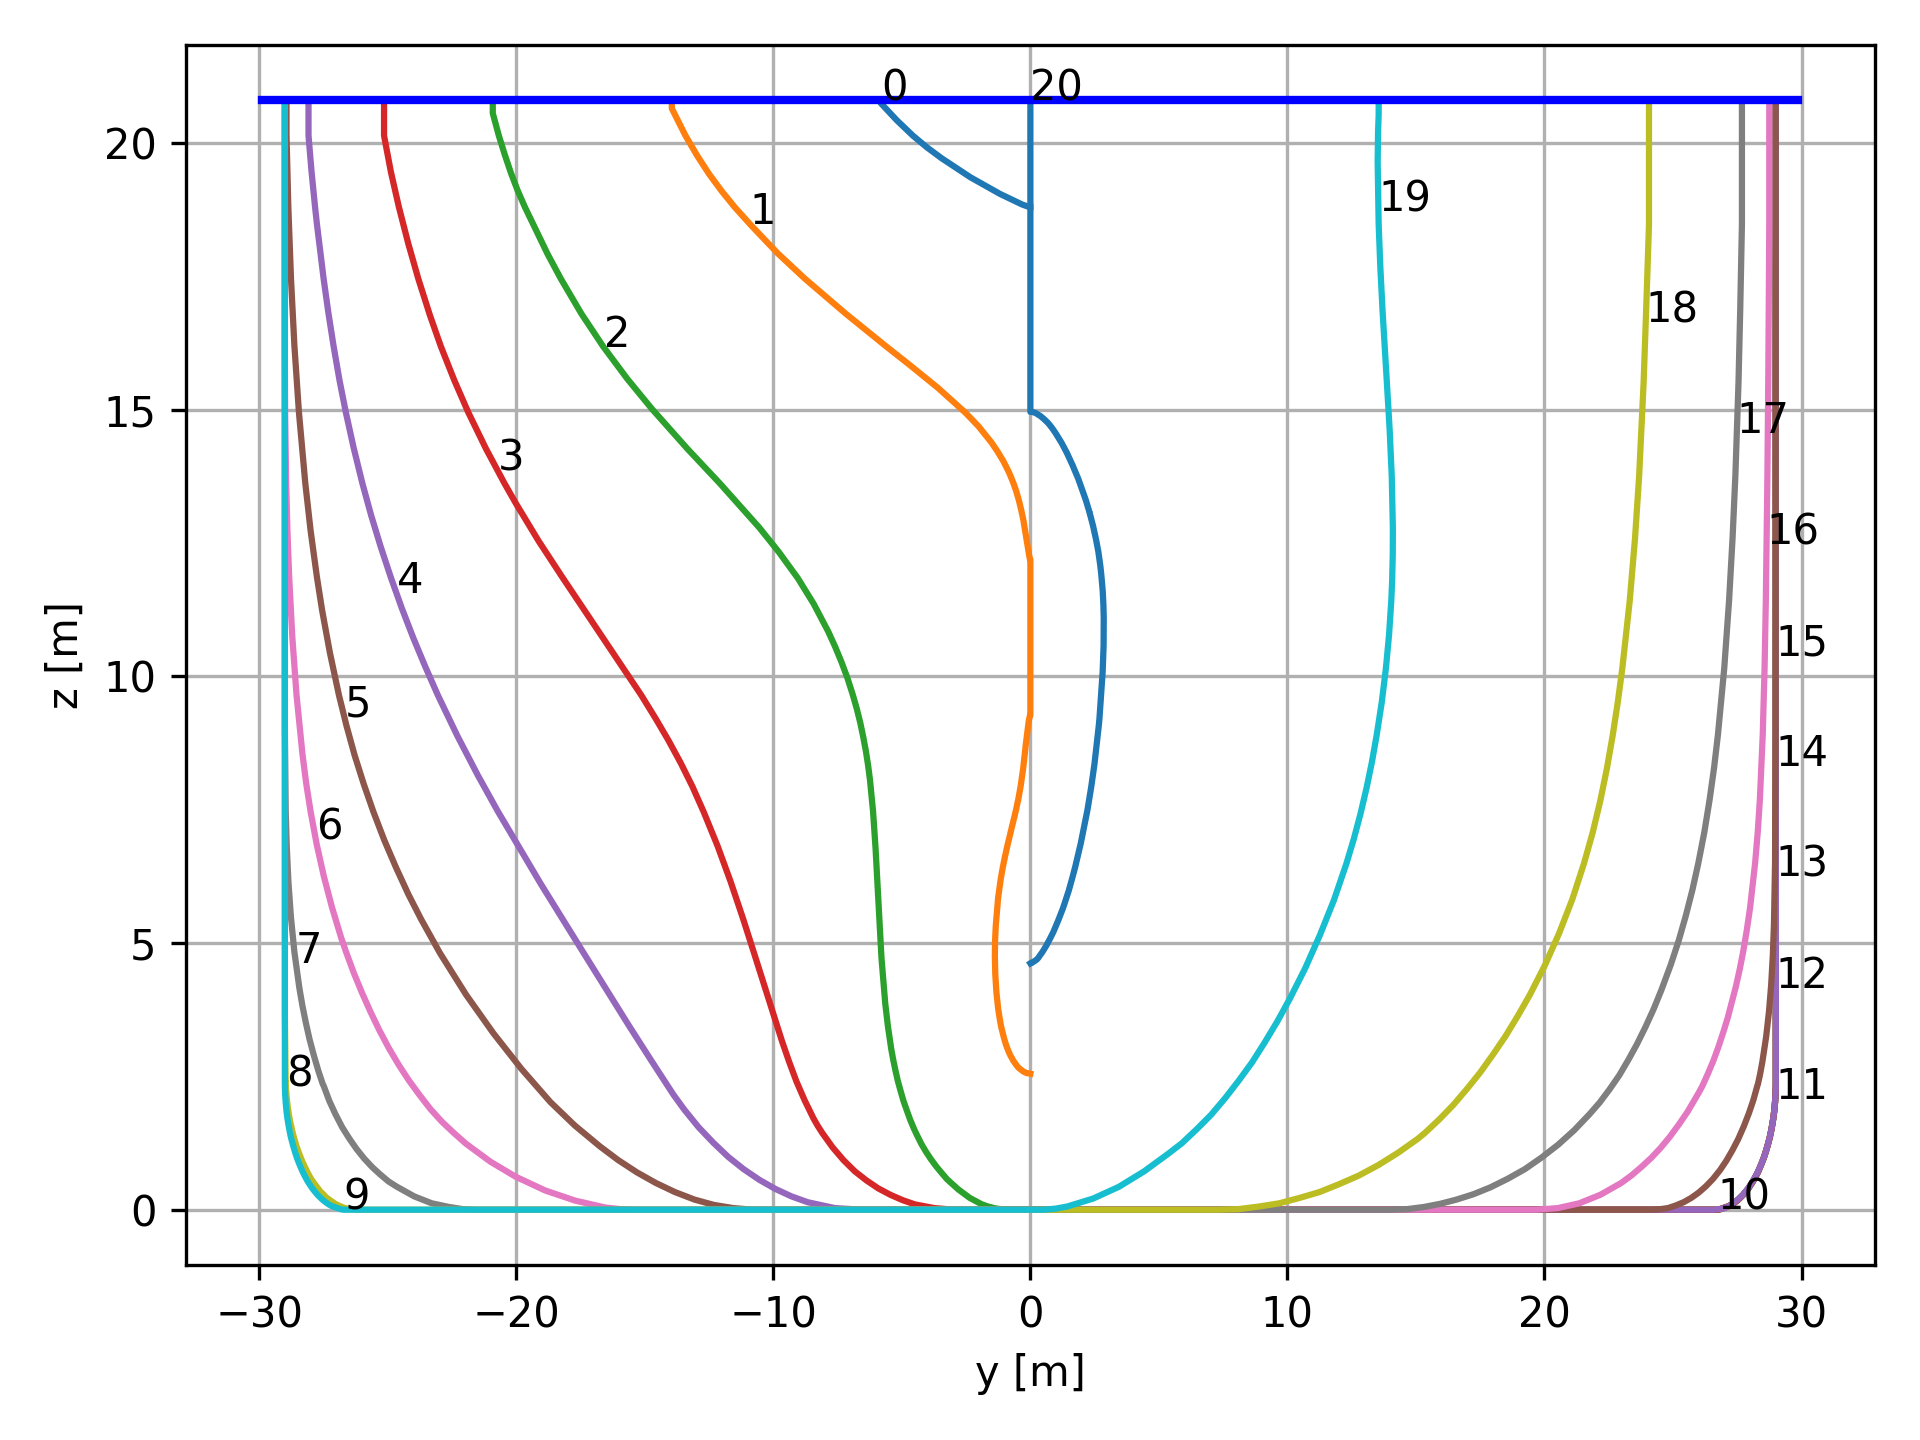
\includegraphics[width = 0.5\textwidth]{figures/body_plan.png}\end{center}
        \vspace{-1cm}
        \caption{KVLCC2 body plan}
        \label{fig:body_plan}
    \end{figure}
    

    